% This file was created with tikzplotlib v0.10.1.
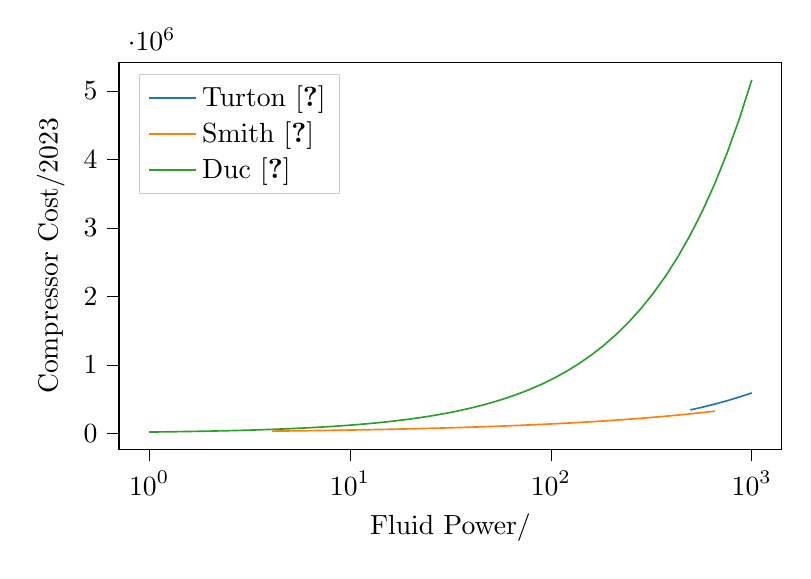
\begin{tikzpicture}

\definecolor{darkgray176}{RGB}{176,176,176}
\definecolor{darkorange25512714}{RGB}{255,127,14}
\definecolor{forestgreen4416044}{RGB}{44,160,44}
\definecolor{lightgray204}{RGB}{204,204,204}
\definecolor{steelblue31119180}{RGB}{31,119,180}

\begin{axis}[
legend cell align={left},
legend style={
  fill opacity=0.8,
  draw opacity=1,
  text opacity=1,
  at={(0.03,0.97)},
  anchor=north west,
  draw=lightgray204
},
log basis x={10},
tick align=outside,
tick pos=left,
unbounded coords=jump,
x grid style={darkgray176},
xlabel={Fluid Power/\unit{\kilo\watt}},
xmin=0.707945784384138, xmax=1412.53754462275,
xmode=log,
xtick style={color=black},
xtick={0.01,0.1,1,10,100,1000,10000,100000},
xticklabels={
  \(\displaystyle {10^{-2}}\),
  \(\displaystyle {10^{-1}}\),
  \(\displaystyle {10^{0}}\),
  \(\displaystyle {10^{1}}\),
  \(\displaystyle {10^{2}}\),
  \(\displaystyle {10^{3}}\),
  \(\displaystyle {10^{4}}\),
  \(\displaystyle {10^{5}}\)
},
y grid style={darkgray176},
ylabel={Compressor Cost/\unit{\USD}2023},
ymin=-239212.588157367, ymax=5417078.03411352,
ytick style={color=black},
ytick={-1000000,0,1000000,2000000,3000000,4000000,5000000,6000000},
yticklabels={\ensuremath{-}1,0,1,2,3,4,5,6},
width=10cm, height=6.5cm
]
\addplot [semithick, steelblue31119180]
table {%
1 nan
1.15139539932645 nan
1.32571136559011 nan
1.52641796717523 nan
1.75751062485479 nan
2.02358964772516 nan
2.32995181051537 nan
2.68269579527973 nan
3.08884359647748 nan
3.55648030622313 nan
4.09491506238043 nan
4.71486636345739 nan
5.42867543932386 nan
6.25055192527397 nan
7.19685673001152 nan
8.28642772854684 nan
9.54095476349994 nan
10.9854114198756 nan
12.648552168553 nan
14.5634847750124 nan
16.7683293681101 nan
19.3069772888325 nan
22.2299648252619 nan
25.5954792269954 nan
29.4705170255181 nan
33.9322177189533 nan
39.0693993705462 nan
44.9843266896945 nan
51.7947467923121 nan
59.6362331659464 nan
68.66488450043 nan
79.060432109077 nan
91.0298177991522 nan
104.811313415469 nan
120.679264063933 nan
138.949549437314 nan
159.985871960606 nan
184.206996932672 nan
212.095088792019 nan
244.205309454865 nan
281.176869797423 nan
323.745754281764 nan
372.759372031494 nan
429.193426012878 nan
494.171336132383 340747.195248809
568.986602901829 381469.865701317
655.128556859551 426302.867534644
754.312006335462 475561.121148082
868.511373751352 529571.374100317
1000 588671.121693816
};
\addlegendentry{Turton \cite{Turton2012}}
\addplot [semithick, darkorange25512714]
table {%
1 nan
1.15139539932645 nan
1.32571136559011 nan
1.52641796717523 nan
1.75751062485479 nan
2.02358964772516 nan
2.32995181051537 nan
2.68269579527973 nan
3.08884359647748 nan
3.55648030622313 nan
4.09491506238043 31249.8601953914
4.71486636345739 33343.5122194582
5.42867543932386 35577.4329925841
6.25055192527397 37961.0201232238
7.19685673001152 40504.3008329516
8.28642772854684 43217.9741387549
9.54095476349994 46113.4558614224
10.9854114198756 49202.926649366
12.648552168553 52499.3832199028
14.5634847750124 56016.6930335582
16.7683293681101 59769.6526313913
19.3069772888325 63774.0498807569
22.2299648252619 68046.7303913556
25.5954792269954 72605.6683809726
29.4705170255181 77470.0422890185
33.9322177189533 82660.3154559642
39.0693993705462 88198.3222080681
44.9843266896945 94107.3597095367
51.7947467923121 100412.285968519
59.6362331659464 107139.624409226
68.66488450043 114317.675450082
79.060432109077 121976.635557301
91.0298177991522 130148.724274711
104.811313415469 138868.319764218
120.679264063933 148172.103427096
138.949549437314 158099.214214495
159.985871960606 168691.413276312
184.206996932672 179993.259641076
212.095088792019 192052.297665876
244.205309454865 204919.257044918
281.176869797423 218648.266218073
323.745754281764 233297.080077205
372.759372031494 248927.322928165
429.193426012878 265604.747730562
494.171336132383 283399.512705858
568.986602901829 302386.476477417
655.128556859551 322645.512984106
754.312006335462 nan
868.511373751352 nan
1000 nan
};
\addlegendentry{Smith \cite{Smith2005}}
\addplot [semithick, forestgreen4416044]
table {%
1 17891.5310367637
1.15139539932645 20084.0635910986
1.32571136559011 22545.2818712075
1.52641796717523 25308.1121928668
1.75751062485479 28409.5158546107
2.02358964772516 31890.9836080487
2.32995181051537 35799.0907234618
2.68269579527973 40186.1200763717
3.08884359647748 45110.7615907737
3.55648030622313 50638.8973962215
4.09491506238043 56844.4832026404
4.71486636345739 63810.5376839499
5.42867543932386 71630.2531065259
6.25055192527397 80408.2420605512
7.19685673001152 90261.9369730964
8.28642772854684 101323.161125697
9.54095476349994 113739.892193582
10.9854114198756 127678.241899292
12.648552168553 143324.678264588
14.5634847750124 160888.520190077
16.7683293681101 180604.737735165
19.3069772888325 202737.095560653
22.2299648252619 227581.681587118
25.5954792269954 255470.868075672
29.4705170255181 286777.758122654
33.9322177189533 321921.177053718
39.0693993705462 361371.275492458
44.9843266896945 405655.819061742
51.7947467923121 455367.248861725
59.6362331659464 511170.607180012
68.66488450043 573812.434464575
79.060432109077 644130.756583605
91.0298177991522 723066.295982442
104.811313415469 811675.056721046
120.679264063933 911142.451755366
138.949549437314 1022799.16145815
159.985871960606 1148138.93553536
184.206996932672 1288838.57649332
212.095088792019 1446780.37199633
244.205309454865 1624077.27621636
281.176869797423 1823101.17705208
323.745754281764 2046514.6273778
372.759372031494 2297306.46482472
429.193426012878 2578831.79661787
494.171336132383 2894856.8843882
568.986602901829 3249609.52943125
655.128556859551 3647835.63246933
754.312006335462 4094862.6845767
868.511373751352 4596671.03865314
1000 5159973.91491938
};
\addlegendentry{Duc \cite{Duc2007}}
\end{axis}

\end{tikzpicture}
